\chapter{Exercises with answers}

\begin{Exercise} [
  title={Coding sequence},
  difficulty={1},
  label={excs},
  origin={G. Valle}
 ]
 
 \begin{figure}[H]
  \centering
  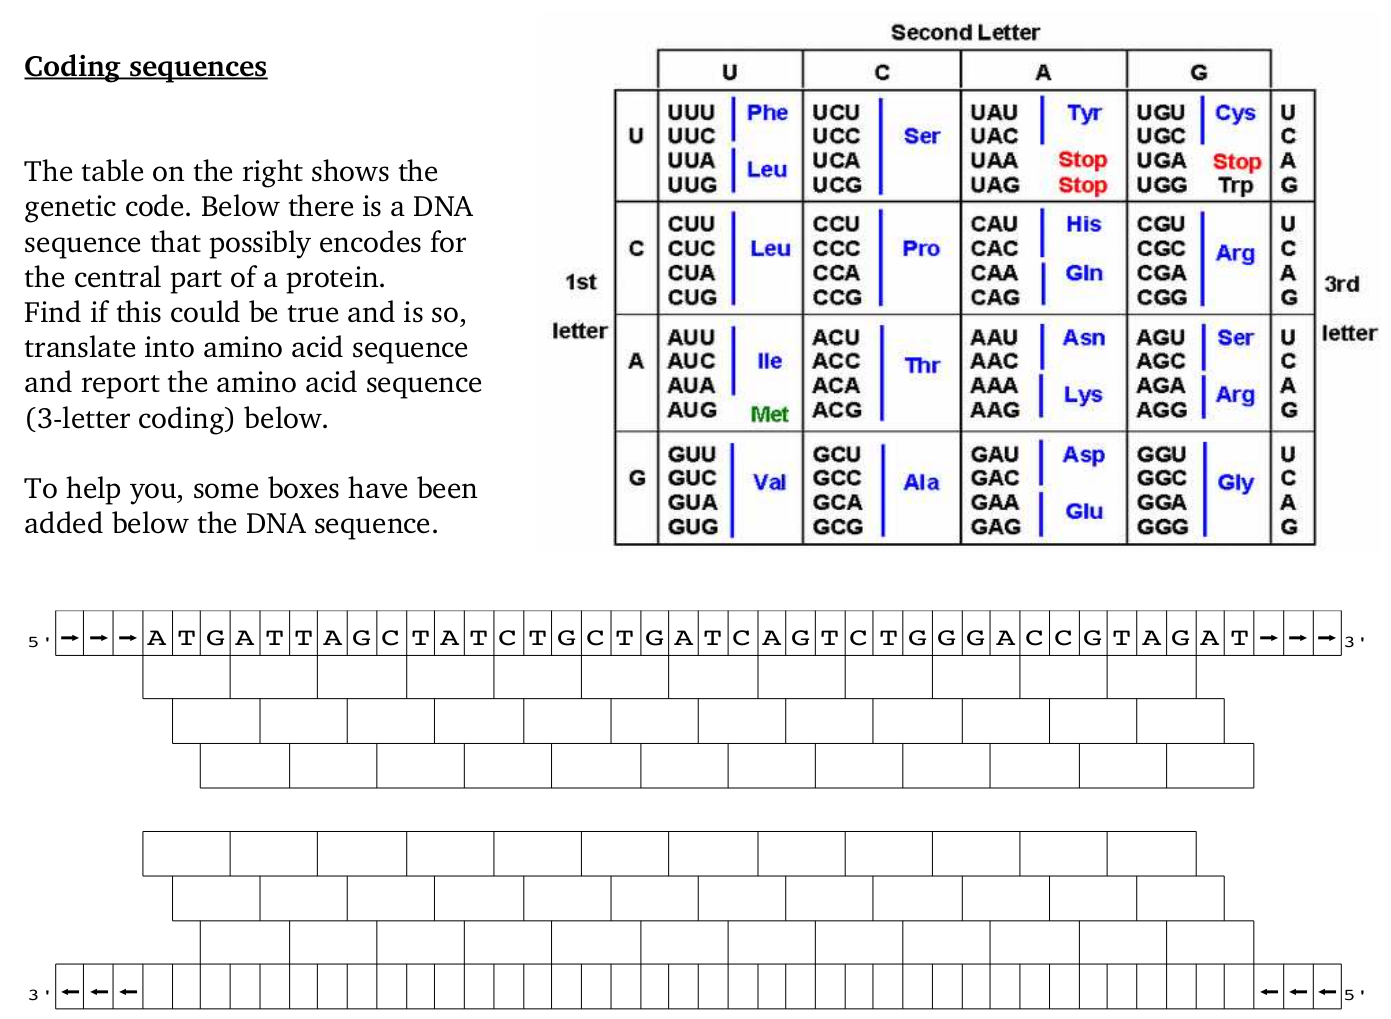
\includegraphics[scale=0.3]{Find_coding_sequence}
 \end{figure}

\end{Exercise}

\newpage

\begin{Answer} [
  ref={excs},
  number={1}
 ]
 
 \begin{figure}[H]
  \centering
  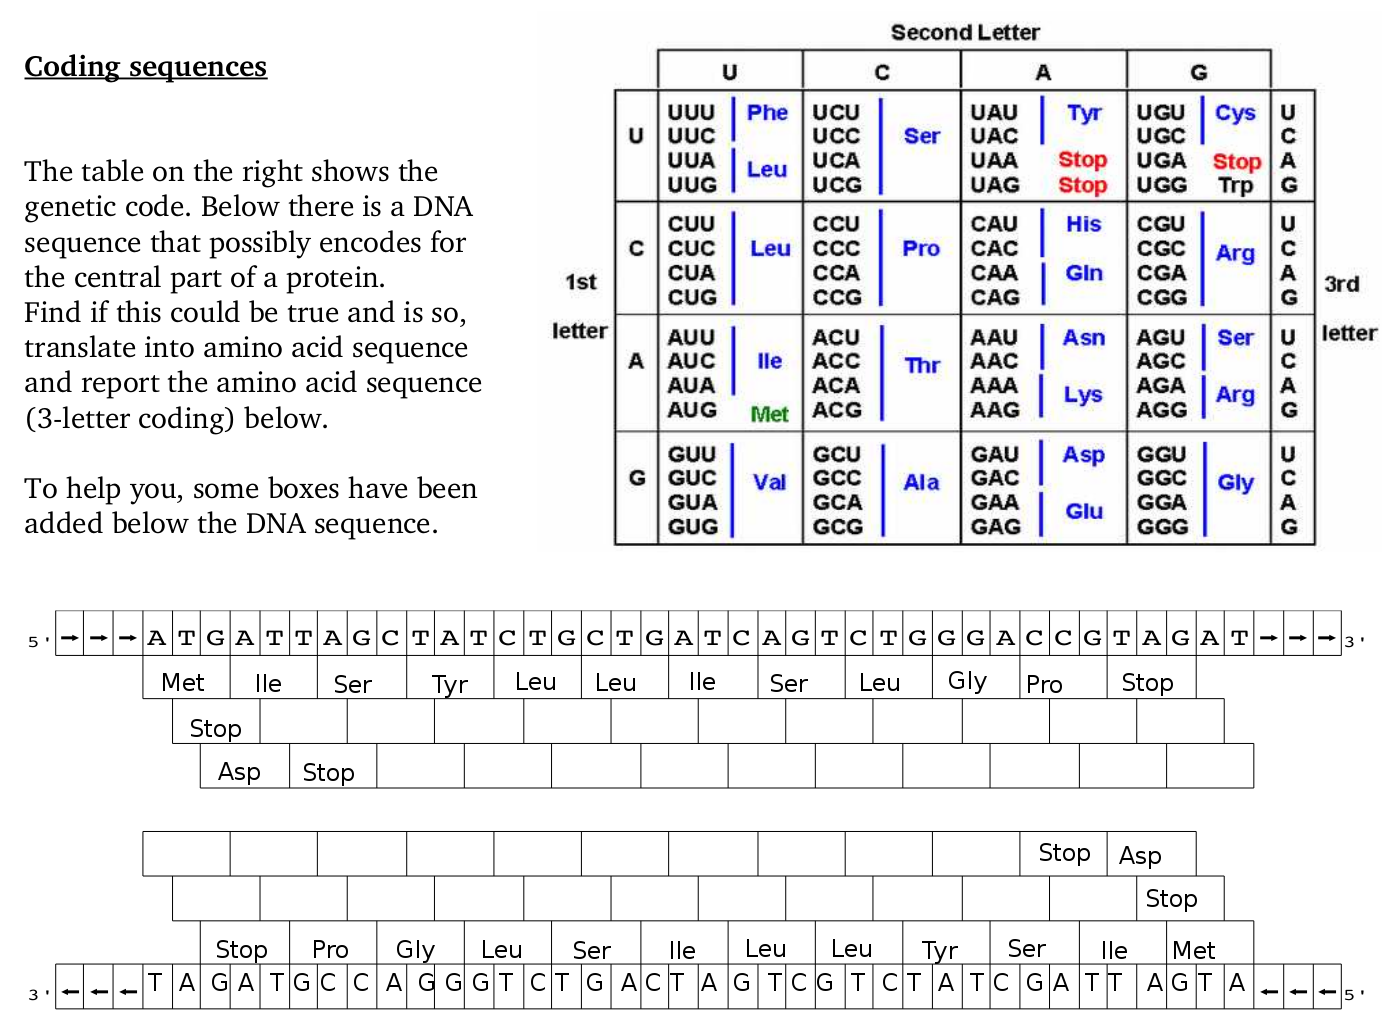
\includegraphics[scale=0.3]{Find_coding_sequence_sol}
 \end{figure}

\end{Answer}



\begin{Exercise} [
  title={Chromosomes},
  difficulty={1},
  label={ex1},
  origin={G. Valle}
 ]

  In adult human cells there are 46 chromosomes. De novo mutations are generally
very rare and we are not considering them in the following reasoning.
Answer \textbf{True} or \textbf{False}:

  \Question 23 chromosome are inherited from the mother and 23 from the father
  \Question Each chromosome of a child must have an identical copy in one of the
2 parents
  \subQuestion Explain why
\end{Exercise}

\begin{Answer} [
   ref={ex1},
   number={1}
 ]

  \Question \textbf{True}
  \Question \textbf{False}
  \subQuestion The second statement is wrong because of the crossing over

\end{Answer}


\begin{Exercise} [
  title={Genomes and genes},
  difficulty={1},
  label={ex2},
  origin={G. Valle}
 ]

  Approximately, how big is the genome and how many genes are there...

  \Question In a bacterium like \textbf{E. Coli}
  \Question In a simple eukaryote like \textbf{yeast}
  \Question In humans

\end{Exercise}

\begin{Answer} [
  ref={ex2},
  number={2}
 ]

  \Question Genome size: 100 Mbp. Number of genes: 19000 (27\% encoding)
  \Question Genome size: 13 Mbp. Number of genes: 6000 (70\% encoding)
  \Question Genome size: 3000 Mbp. Number of genes: 23000/25000 (1.5\% encoding)

\end{Answer}

\begin{Exercise} [
  title={Enzyme},
  difficulty={1},
  label={ex3},
  origin={G. Valle}
 ]

  Answer the questions.

  \Question How is called the enzyme that duplicate the DNA?
  \Question How is called the enzyme that transcribes DNS into RNA?
  \Question How is it called the biological structure where proteins are
synthesized?
\end{Exercise}

\begin{Answer} [
  ref={ex3},
  number={3}
 ]

  \Question DNA Polymerase
  \Question RNA Polymerase
  \Question Ribosome
\end{Answer}

\begin{Exercise} [
  title={Smith and Waterman algorithm},
  difficulty={1},
  label={exSW},
  origin={G. Valle}
 ]
 
 Consider the following two sequences:

 \begin{itemize}
  \item \texttt{DFTLNL}
  \item \texttt{EYSHMC}
 \end{itemize}

 Simulate the Smith-Waterman algorithm using the PAM240 and a gap penalty of
 4 points, both for starting and extending the gap.
 Finally, report the two aligned sequences below and the final score of the
 alignment.

 \begin{figure}[H]
  \centering
  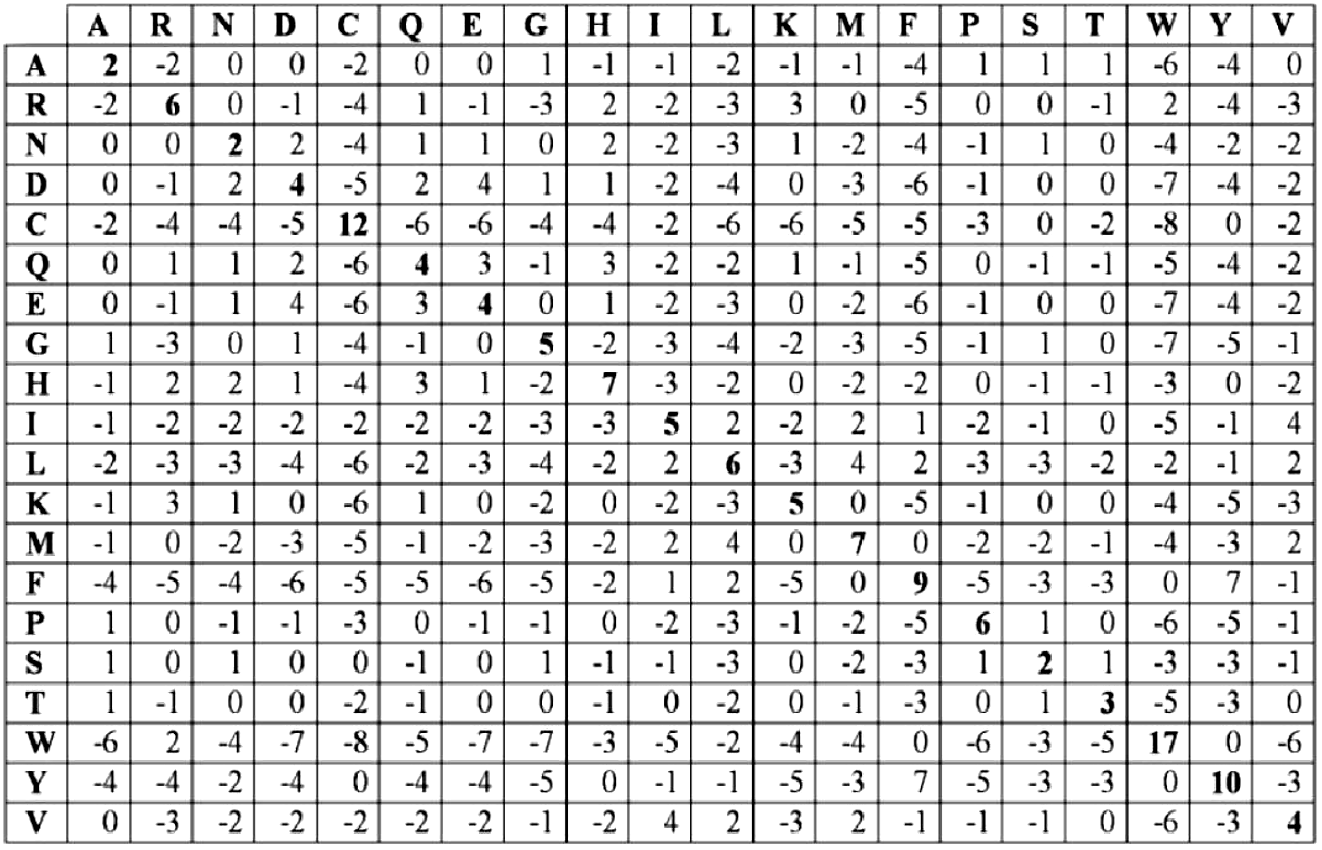
\includegraphics[scale=0.3]{PAM240}
 \end{figure}

\end{Exercise}

\newpage

\begin{Answer} [
  ref={exSW},
  number={4}
 ]
 
 The scoring matrix obtained by applying the algorithm is the following: 

 \begin{figure}[H]
  \centering
  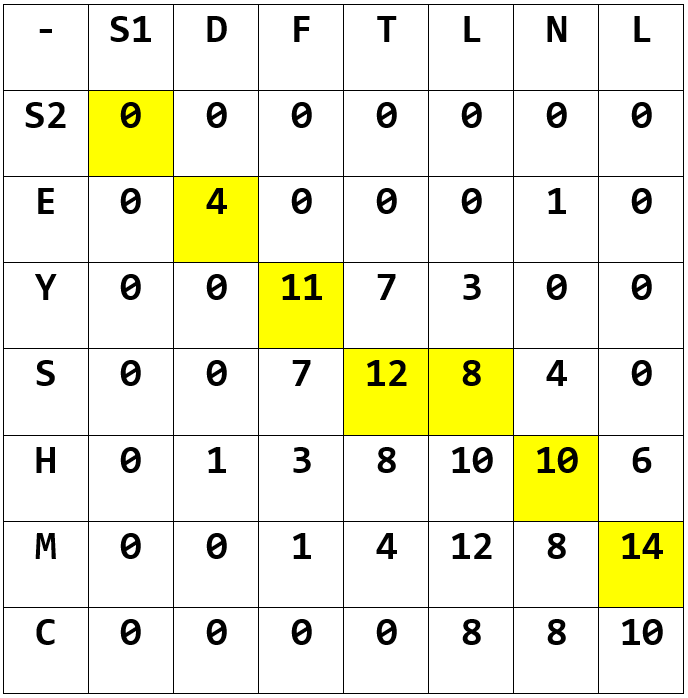
\includegraphics[scale=0.3]{matrix_ex}
 \end{figure}

 The \textbf{final alignment} is:

 \begin{figure}[H]
  \centering
  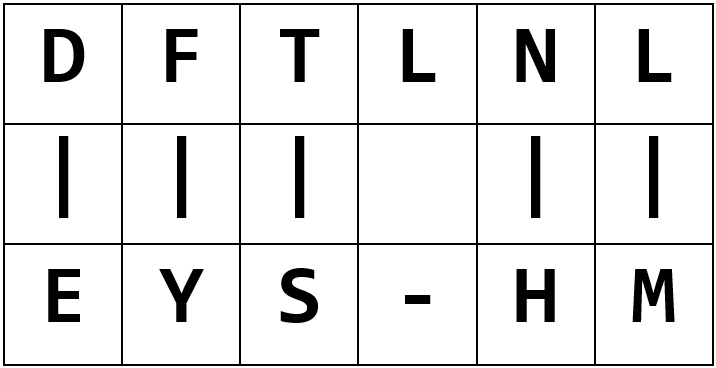
\includegraphics[scale=0.2]{alignment_ex}
 \end{figure}

 Thus, the \textbf{final score} is 14.

\end{Answer}

\section{Quiz}

\subsection{Flow of the genetic information}

\begin{Exercise} [
  title={Mitosis},
  difficulty={1},
  label={ex7},
  origin={G. Valle}
 ]

Answer \textbf{True} or \textbf{False}:

  \Question Mitosis is a process essential in the duplication of genetic
information of somatic cells.
Typically a diploid cell (2N) duplicates its DNA to become 4N, then the
chromosomes separate in two daughter diploid cells.

\end{Exercise}

\begin{Exercise} [
  title={Meiosis},
  difficulty={1},
  label={ex8},
  origin={G. Valle}
 ]

  \Question When we talk about DNA content in an eukaryotic cell, we refer to
N to indicate the DNA content.
Therefore we say that a haploid cell is 'N' and a diploid cell is '2N'.

Meiosis is a process essential in distributing genetic information in germinal
cells. What happens during  meiosis ?

Choose an alternative:

\begin{enumerate}
  \item During meiosis,  a diploid cell (2N) duplicates its DNA to become 4N,
then there are two cell divisions without DNA duplication, producing 4 haploid
cells called “gametes”, each with N chromosomes.
  \item The entire process of meiosis starts from a diploid cell (2N) that
divides itself into two haploid cells (N) called “gametes”, each with N
chromosomes.
\end{enumerate}

\end{Exercise}

\begin{Exercise} [
  title={Crossing-Over (1)},
  difficulty={1},
  label={ex9},
  origin={G. Valle}
 ]

Answer \textbf{True} or \textbf{False}:

  \Question Crossing over is a genetic process that is important in evolution
because it creates new mutations

\end{Exercise}

\begin{Exercise} [
  title={Crossing-Over (2)},
  difficulty={1},
  label={ex10},
  origin={G. Valle}
 ]

  \Question When does crossing over occurs?

Choose an alternative:

\begin{enumerate}
  \item It occurs during mitosis.
  \item It occurs during meiosis.
  \item It occurs at every cell duplication.
\end{enumerate}

\end{Exercise}

\begin{Exercise} [
  title={Eukaryotes},
  difficulty={1},
  label={ex11},
  origin={G. Valle}
 ]

Answer \textbf{True} or \textbf{False}:

  \Question Eukaryotes alternate haploid and diploid generations

\end{Exercise}

\begin{Exercise} [
  title={Haploidy},
  difficulty={1},
  label={ex12},
  origin={G. Valle}
 ]

Answer \textbf{True} or \textbf{False}:

  \Question The haploid status is predominant in most eukaryotes

\end{Exercise}

\begin{Exercise} [
  title={Diploidy},
  difficulty={1},
  label={ex13},
  origin={G. Valle}
 ]

Answer \textbf{True} or \textbf{False}:

  \Question Diploidy is important in evolution because it helps to eliminate
bad genes.

\end{Exercise}

\subsection{Answers (Flow of the genetic information)}

\begin{Answer} [
   ref={ex7},
   number={7}
 ]

  \Question \textbf{True}

\end{Answer}

\begin{Answer} [
   ref={ex8},
   number={8}
 ]

  \Question 1

Typically, during meiosis,  a diploid cell (2N) duplicates its DNA to become
4N, then there are two cell divisions without DNA duplication, producing 4
haploid cells called “gametes", that are 1N.

\end{Answer}

\begin{Answer} [
   ref={ex9},
   number={9}
 ]

  \Question \textbf{False}

\end{Answer}

\begin{Answer} [
   ref={ex10},
   number={10}
 ]

  \Question 2

\end{Answer}

\begin{Answer} [
   ref={ex11},
   number={11}
 ]

  \Question \textbf{True}

It is true. For instance in mammals, there is the alternation between the
diploid phase (that is hugely predominant and multicellular) with the haploid
stage that is unicellular, represented by the egg and the spermatozoon.
The two haploid gametes join during fertilization to produce a diploid cell
that by means of many cell duplications (mitosis) will generate the fully
developed diploid organism.
Some specialized organs (gonads) are responsible to host the process of
gametogenesis where the haploid gametes are produced by meiosis.  

\end{Answer}

\begin{Answer} [
   ref={ex12},
   number={12}
 ]

  \Question \textbf{False}

\end{Answer}

\begin{Answer} [
   ref={ex13},
   number={13}
 ]

  \Question \textbf{False}

\end{Answer}

\subsection{DNA Sequencing}

\begin{Exercise} [
  title={NGS},
  difficulty={1},
  label={ex14},
  origin={G. Valle}
 ]

Answer \textbf{True} or \textbf{False}:

  \Question There are several technologies for DNA sequencing.
The so called Next Generation Sequencing technologies, like Illumina, are able
to produce hundreds of million reads, but only from very short fragments of
DNA, a few hundred bases long. 

\end{Exercise}

\begin{Exercise} [
  title={Sanger Sequencing},
  difficulty={1},
  label={ex15},
  origin={G. Valle}
 ]

Answer \textbf{True} or \textbf{False}:

  \Question The Sanger sequencing technology has been very important in the
past, but now is obsolete and the Sanger DNA sequencers are not anymore
available on the market.

\end{Exercise}

\begin{Exercise} [
  title={DNA Analysis},
  difficulty={1},
  label={ex16},
  origin={G. Valle}
 ]

A DNA locus has been sequenced both from father and mother.
The results show that one base is different (shown by the arrow).

 \begin{figure}[H]
  \centering
  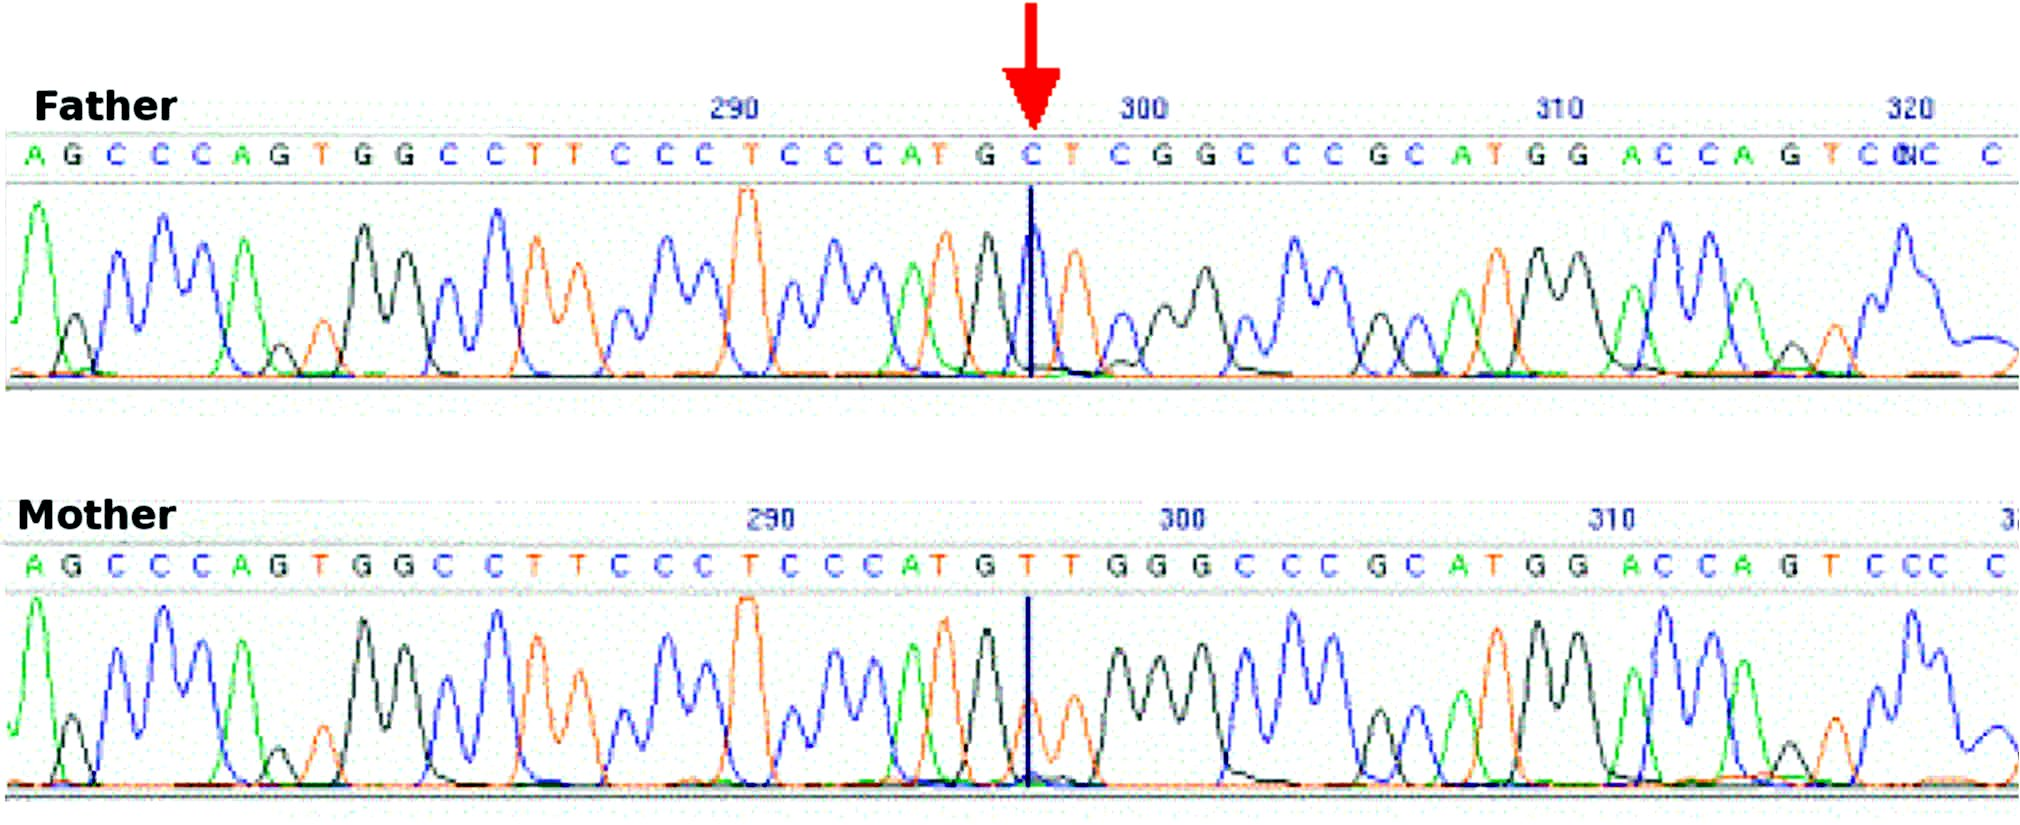
\includegraphics[scale=0.2]{sanger1}
 \end{figure}

Choose an alternative:

\begin{enumerate}
  \item Both father and mother are homozygous.
  \item Both father and mother are heterozygous.
  \item Their child will be heterozygous.
  \item Their child will be homozygous.
  \item The child could be either homo or heterozygous depending on the
chromosomal re-assortment.
\end{enumerate}

\end{Exercise}

\begin{Exercise} [
  title={Sequence coverage},
  difficulty={1},
  label={ex17},
  origin={G. Valle}
 ]

  \Question A genome of 5 million bases (5 Mbp) has been shotgun sequenced
using mate pair reads.

The DNA fragments average 10000 bp and the reads average 500 bases.
A total of 10000 reads were produced (5000 pairs). Estimate the average
\textbf{sequence coverage}.

\end{Exercise}

\begin{Exercise} [
  title={Physical coverage},
  difficulty={1},
  label={ex18},
  origin={G. Valle}
 ]

  \Question A genome of 5 million bases (5 Mbp) has been shotgun sequenced
using mate pair reads.

The DNA fragments average 10000 bp and the reads average 500 bases.
A total of 10000 reads were produced (5000 mates pairs). Estimate the average
\textbf{physical coverage}.

\end{Exercise}

\begin{Exercise} [
  title={Mate pairs},
  difficulty={1},
  label={ex19},
  origin={G. Valle}
 ]

A mate pairs library was sequenced and mapped on a reference genome.
The 3 tracks shown in the figure show a particular region of the genome.
What do you think is there?

 \begin{figure}[H]
  \centering
  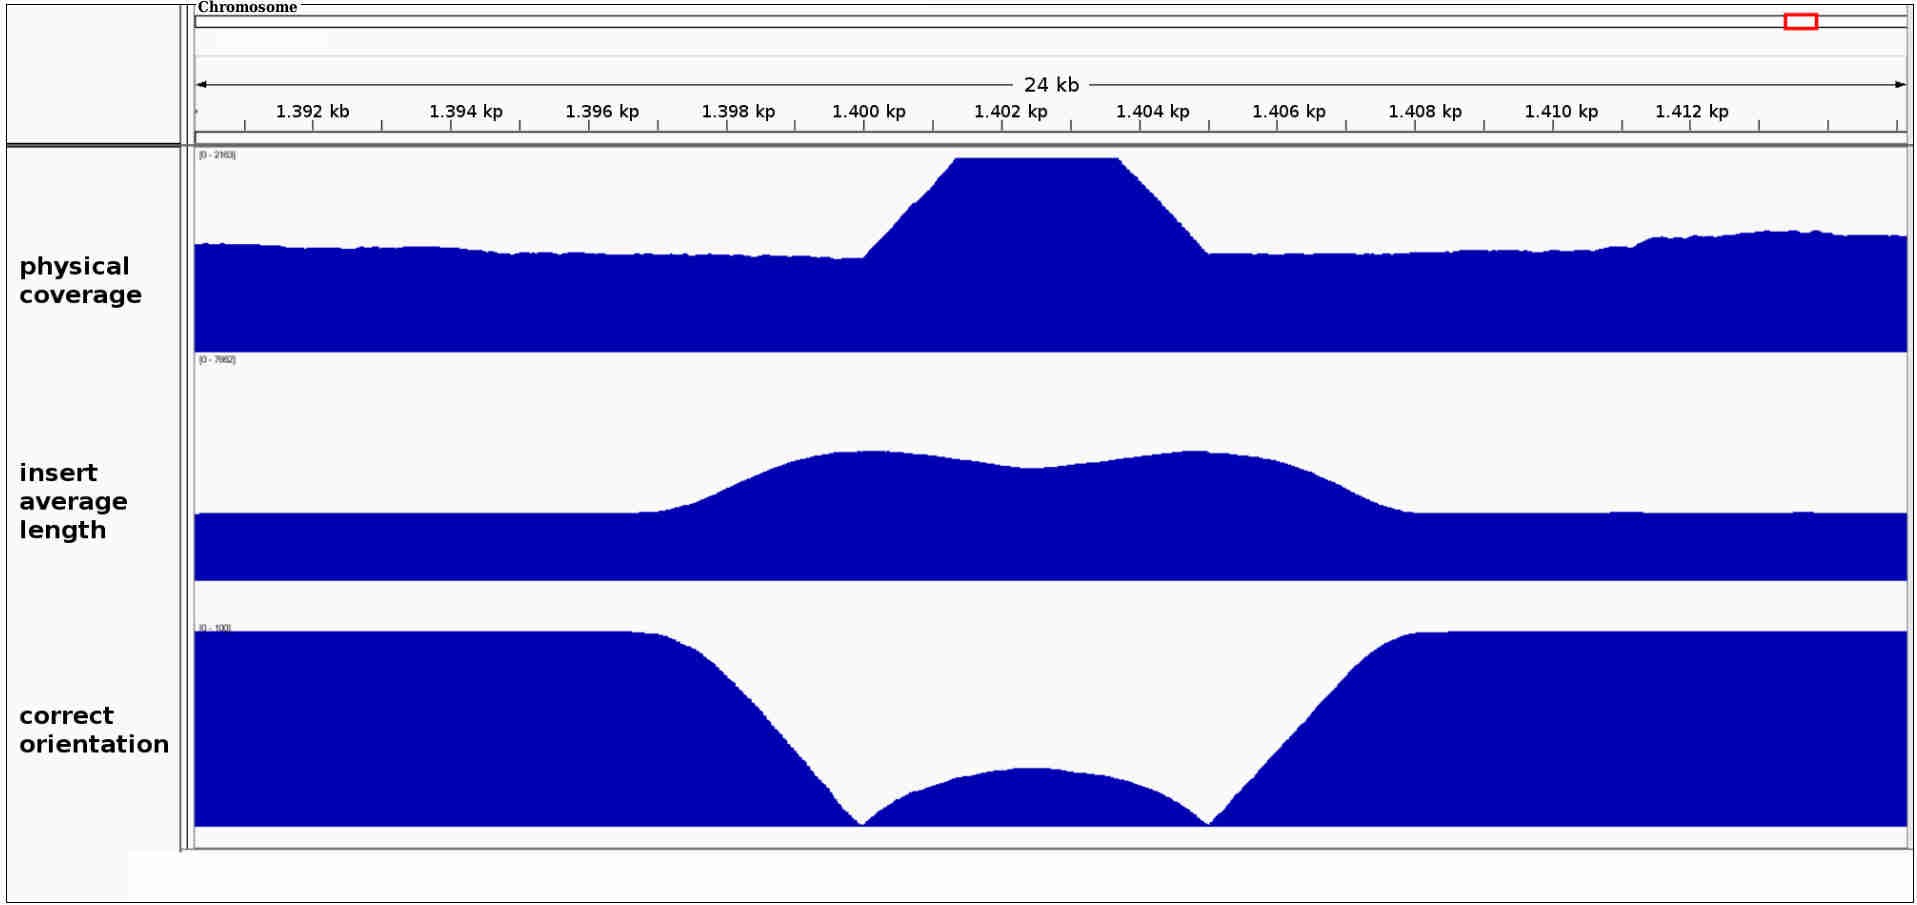
\includegraphics[scale=0.2]{tracks}
 \end{figure}

Choose an alternative:

\begin{enumerate}
  \item long deletion.
  \item short deletion.
  \item long insertion.
  \item long inversion.
  \item short insertion.
  \item short inversion
\end{enumerate}

\end{Exercise}

\subsection{Answers (DNA Sequencing)}

\begin{Answer} [
   ref={ex14},
   number={14}
 ]

  \Question \textbf{True}

\end{Answer}

\begin{Answer} [
   ref={ex15},
   number={15}
 ]

  \Question \textbf{False}

Sanger sequencing is still very important and there are still Sanger DNA
sequencers on the market.

For instance, if you want to sequence a short piece of DNA, you don't need
million reads!

Furthermore, there are many DNA sequencing services that will do everything
for you: you supply the DNA, for instance a fragment amplified by PCR, and
they give you the sequence at a cost of less than 5 euro.

\end{Answer}

\begin{Answer} [
   ref={ex16},
   number={16}
 ]

  \Question 1,3

In the case of heterozygosity we would see two different color peaks
overlapping as shown below.
Instead we see that at the given locus the father shows a C and the mother
a T, both in homozygosity.
The father will pass to the child the C allele and the mother the T allele.
Therefore the child will be certainly heterozygous carrying both alleles.

The correct answer is \textbf{Both father and mother are homozygous,
their child will be heterozygous}

\end{Answer}

\begin{Answer} [
   ref={ex17},
   number={17}
 ]

  \Question 1

\textbf{Formula} The average coverage for a whole genome can be calculated
from the length of the original genome (G), the number of reads (N), and the
average read length (L) as $N*L/G$

\end{Answer}

\begin{Answer} [
   ref={ex18},
   number={18}
 ]

  \Question 0.5

\end{Answer}

\begin{Answer} [
   ref={ex19},
   number={19}
 ]

  \Question 4 (long inversion)

\end{Answer}

\subsection{Others questions}

\begin{Exercise} [
  title={mRNA},
  difficulty={1},
  label={ex20},
  origin={G. Valle}
 ]

Answer \textbf{True} or \textbf{False}:

  \Question The mature mRNA is encoding proteins by means of codons that are
3 bases long. Therefore mRNA have lengths that are necessarily multiple of 3.

\end{Exercise}

\begin{Exercise} [
  title={Splicing},
  difficulty={1},
  label={ex21},
  origin={G. Valle}
 ]

Answer \textbf{True} or \textbf{False}:

  \Question Many genes contain introns that must be removed to obtain a
functional mRNA (splicing process).
The splicing mechanism is performed by the enzyme RNA polymerases that
recognizes the introns and transcribes into mRNA only the exons.
As a result the mRNA is constituted only by the exons.

\end{Exercise}

\begin{Exercise} [
  title={Objective function for alignment},
  difficulty={1},
  label={ex22},
  origin={G. Valle}
 ]

\begin{equation}
Score = \sum_{i=1}^{L} s(a_i,b_i) - \sum_{j=1}^{G} (\gamma + \delta(len(j)-1))
\end{equation}

  \Question Explain what these symbols represent: L, G, $\gamma$, $\delta$,
$s(a_i,b_i)$

\end{Exercise}

\subsection{Others answers}

\begin{Answer} [
   ref={ex20},
   number={20}
 ]

  \Question \textbf{False}

Although the coding regions have a length that must be multiple of 3, there are untranslated regions both in 3' and 5' (respectively 3'UTR and 5'UTR) that can be any length. Therefore the mRNA is not necessarily a multiple of 3.

\end{Answer}

\begin{Answer} [
   ref={ex21},
   number={21}
 ]

  \Question \textbf{False}

RNA polymerases transcribe into RNA the full length of a gene, including the introns. The splicing process acts on the transcribed RNA by removing the intronic portions.

\end{Answer}

\begin{Answer} [
   ref={ex22},
   number={22}
 ]

  \Question L – length of the alignment, $\delta$ – penalty for gap elongation,
G – number of gaps, $\gamma$ – penalty for staring a gap, $s(a_i, b_i)$ –
score of the match at position i.

\end{Answer}
